\documentclass[journal]{IEEEtran}



% All authors of accepted papers are entitled to 10 pages free of charge (in two-column format, including title, abstract, all figures, tables, references, biographies and author pictures)



% *** GRAPHICS RELATED PACKAGES ***
%
% \ifCLASSINFOpdf
  % \usepackage[pdftex]{graphicx}
  % declare the path(s) where your graphic files are
  % \graphicspath{{../pdf/}{../jpeg/}}
  % and their extensions so you won't have to specify these with
  % every instance of \includegraphics
  % \DeclareGraphicsExtensions{.pdf,.jpeg,.png}
% \else


% \hyphenation{op-tical net-works semi-conduc-tor}
\usepackage{graphicx} 
\usepackage{kotex}
\usepackage{array} % 표의 기능을 확장하는 패키지
% 'L' 열 타입을 정의 (지정된 너비 내에서 왼쪽 정렬)
\newcolumntype{L}[1]{>{\raggedright\let\newline\\\arraybackslash\hspace{0pt}}m{#1}}


\begin{document}
\title{NetAgent: A Multi-Agent System for Network Management}


\author{
Hyeonjeong Lee$^{1}$, Yujin Park$^{2}$,Jinyeong Park$^{3}$, Cheoneum Park$^{1}$\footnotemark[*] \\
Hanbat National Univ.$^{1}$, Chungnam National Univ.$^{2}$, Sungkyunkwan Univ.$^{3}$\\ 
leehj@edu.hanbat.ac.kr, newmail@cnu.ac.kr, jy.bak@skku.edu, parkce@hanbat.ac.kr

% \thanks{M. Shell was with the Department
% of Electrical and Computer Engineering, Georgia Institute of Technology, Atlanta,
% GA, 30332 USA e-mail: (see http://www.michaelshell.org/contact.html).}% <-this % stops a space
% \thanks{J. Doe and J. Doe are with Anonymous University.}% <-this % stops a space
% \thanks{Manuscript received April 19, 2005; revised August 26, 2015.}
}


\markboth{IEEE TRANSACTIONS ON NETWORK AND SERVICE MANAGEMENT, VOL 00, NO. 0, February 2026}%
{Shell \MakeLowercase{\textit{et al.}}: Bare Demo of IEEEtran.cls for IEEE Journals}



% make the title area

\maketitle

\begin{abstract}
    네트워크 인프라의 규모 확장과 서비스 다양화로 인해 네트워크 구성 및 운영의 복잡성이 급격히 증가하고 있다. 이에 따라 운영 효율성을 향상시키고 관리 부담을 줄이기 위한 네트워크 관리 자동화 기술이 요구되고 있다. 이 과정에서 Large Language Models(LLM)을 네트워크 관리 도메인에 적용하려는 연구가 활발히 이루어지고 있다. 그렇다면 LLM은 네트워크 설정 파일을 얼마나 정확하게 해석하고 분석할 수 있는가? 기존 벤치마크는 표준 문서의 지식 회상이나 설정 생성에 치중하여 이 질문에 답하기 어렵다. 본 연구는 벤치마크, 평가 지표, 도구 통합 시스템을 하나의 프레임워크로 제안한다. NetConfigQA~2.0은 설정 파일과 Batfish 시뮬레이션을 결합한 이중 경로 파이프라인을 통해 5단계 인지 난이도의 QA 쌍을 자동 생성하며, 설정 파일과 정책 파일만 교체하면 토폴로지 규모에 관계없이 데이터셋이 확장된다. 답변 타입별 정답 구조를 반영하는 Type-Aware Accuracy(TA-Acc)를 도입하여 네트워크 데이터의 평가 문제를 다룬다. 4개 토폴로지(10\textasciitilde40 노드, 총 9,462 QA)와 6개 LLM을 평가한 결과, 사실 추출(L1\textasciitilde L3)에서는 모델 간 차이가 뚜렷하나 경로 추론과 장애 분석(L4/L5)에서는 모든 모델이 시뮬레이션 장벽에 직면하였다. 이 한계를 다루기 위해 도구 통합 Multi-Agent 시스템 NetAlly를 제시하고, Single LLM $\rightarrow$ Pure MAS $\rightarrow$ NetAlly의 3-way 비교를 통해 성능 향상의 주된 원천이 에이전트 구조가 아닌 네트워크 분석 도구의 통합에 있음을 보인다. 또한, 오류 진단, 도달 가능성 검증, 구성 합성 등의 복잡한 작업을 능동적으로 수행하도록 설계하여 실제 네트워크 운영 환경을 반영한 평가를 통해 자동화 수행 능력과 정확도를 검증하였다. 이를 통해 NetAgent가 네트워크 관리 분야에서 실질적인 적용 가능성을 가진다는 것을 입증하며, 향후 네트워크 관리 시스템 구현의 기반이 되는 기술로 활용될 수 있음을 제시한다.
\end{abstract}

% Note that keywords are not normally used for peerreview papers.
\begin{IEEEkeywords}
  Network Configuration Interpretation, Network Management, Multi-Agent System, Benchmark, 정형 검증, Batfish, Type-Aware Accuracy. 
\end{IEEEkeywords}


\IEEEpeerreviewmaketitle

\section{Introduction}
\IEEEPARstart{최}{최근} 인프라의 급격한 발전과 클라우드 컴퓨팅, 소프트웨어 정의 네트워킹(SDN), 네트워크 기능 가상화(NFV), 그리고 대규모 분산 서비스의 확산은 네트워크 환경의 복잡성을 기하급수적으로 증가시키고 있다. 현대 네트워크는 다양한 프로토콜, 이기종 장비, 동적 트래픽 패턴, 그리고 빈번한 구성 변경을 포함하고 있어 관리 난이도가 지속적으로 증가하고 있다. 기존의 수동 기반 네트워크 관리 방식은 운영자의 경험과 반복적인 수작업에 의존하고 있어 구성 오류 가능성이 높고, 장애 발생 시 신속한 대응이 어려우며, 대규모 네트워크 환경에서 확장성 측면에서도 한계를 가진다\cite{mao2017neural, meng2020interpreting}.

초기 네트워크 자동화 연구는 스크립트 기반 자동화나 정책 기반 관리 기법을 중심으로 발전해 왔으며, 최근에는 머신러닝 기반 접근 방식이 네트워크 이상 탐지, 트래픽 예측, 구성 검증 등 다양한 영역에 적용되고 있다. 특히 자연어 이해와 추론 능력을 갖춘 거대 언어 모델(Large Language Models, LLM)은 복잡한 네트워크 구성 문서를 분석하고, 운영자의 질의를 해석하며, 자동으로 구성 명령을 생성할 수 있는 가능성을 보여주면서 네트워크 관리 분야에서 새로운 패러다임으로 주목받고 있다\cite{liu2025large, wu2024netllm}. LLM은 기존 방법으로는 다루기 어려웠던 비정형 데이터 처리와 코드 생성, 다단계 추론 등에서 높은 성능을 보이며 다양한 실무 태스크로 빠르게 확장되고 있다.~\cite{ref1, ref4, ref27}. 

그러나 기존의 단일 LLM 기반 접근 방식은 네트워크 환경에서 요구되는 높은 신뢰성과 정확성을 보장하는 데 한계를 가진다\cite{mondal2023llm_router, wang2025network_arena}. 특히 네트워크는 외부 도구와의 연동, 동적 환경 인식, 긴 컨텍스트에 걸친 정밀 추론은 단순한 텍스트 생성보다 더 복합적인 조정 과정을 요구하기 때문에 단일 LLM은 복잡한 설정 간 관계나 과정을 완전히 이해하지 못하거나, 근거가 부족한 정보를 생성하는 hallucination 문제를 발생시킬 가능성이 있다\cite{bekri2025bridging, wang2024netconfeval}. 

이러한 한계를 여러 에이전트가 역할을 분담해 태스크를 처리하는 Multi-Agent System(MAS) 접근이 확산되고 있으며~\cite{ref2, arzo2021multiagent, bimo2025intentbased}, LangGraph~\cite{ref3} 등의 프레임워크가 에이전트 간 상태 관리와 도구 호출을 체계화하고 있다.
최근에는 도메인 특화 사전학습~\cite{ref18}, LLM 생성 코드 기반 자동화~\cite{ref19}, 네트워크 태스크 적응 프레임워크~\cite{ref31} 등 다양한 접근이 제안되었고, NetConfEval~\cite{wang2024netconfeval}, NIKA~\cite{wang2025network_arena}, NetPress~\cite{ref7}, 그리고 IETF의 NetConfBench 초안~\cite{ref8}은 평가 방법론을 구체화하고 있다. 이는 네트워크 분야에서도 더 이상 LLM의 가능성 자체를 묻는 단계에 머물지 않고, 어떤 태스크를 어떤 방식으로 평가하고 보완할 것인가가 중요한 문제로 이동하고 있음을 보여준다.

대부분의 기존 벤치마크는 \textbf{지식 검색(Knowledge Retrieval)}에 집중한다. TeleQnA~\cite{ref9}는 3GPP 표준 문서에서 사실을 회상하는지, NetBench~\cite{ref11}는 전문가 큐레이션 지식을 활용하는지를 평가한다. 이는 실제 설정 파일에서 네트워크가 어떻게 동작하는지를 추론하는 \textbf{동작 추론(Behavioral Inference)}과는 별개의 문제이다. \texttt{.cfg} 파일에 ``PE1의 OSPF cost가 10''이라고 명시된 것을 읽는 것(L1)과, 그 설정에 따라 PE1에서 PE2까지의 실제 패킷 경로를 추론하는 것(L4)은 질적으로 구분되는 인지 능력을 요구한다.

이 질문에 체계적으로 답하려면 세 가지 조건이 필요하다. 첫째, 사실 추출부터 경로 추론, 장애 영향 분석까지 인지 난이도를 구분하는 벤치마크가 있어야 한다. 기존 벤치마크는 데이터 플레인 시뮬레이션 능력을 측정하지 않는다. 둘째, 네트워크 데이터에 적합한 평가 지표가 필요하다. BERTScore는 \texttt{10.0.1.1}과 \texttt{10.0.1.10}에 0.9 이상의 유사도를 부여하고, Exact Match는 \texttt{\{r1, r2\}}와 \texttt{\{r2, r1\}}을 오답으로 처리하는 등 구조화된 네트워크 답변에 부적합하다. 셋째, 토폴로지의 크기와 복잡도에 따라 LLM의 해석 능력이 달라지므로, 매번 수작업으로 데이터셋을 구성하는 대신 설정 파일만으로 QA를 자동 생성하는 파이프라인이 요구된다.

본 연구는 하나의 연구 질문을 중심으로 전개된다: \textbf{LLM은 네트워크 설정 파일을 얼마나 정확하게 해석하고 분석할 수 있는가?} 이에 답하기 위해 먼저 벤치마크를 구축하고, 평가 과정에서 드러난 한계를 도구 통합 시스템으로 다루며, 그 결과를 실증적으로 분석한다.

본 연구의 기여는 다음과 같다.
\begin{itemize}
  \item \textbf{C1.} \emph{벤치마크, 자동 생성 파이프라인, 평가 지표.} 실제 설정 파일로부터 5단계 인지 난이도의 QA 쌍을 자동 생성하는 벤치마크 NetConfigQA~2.0을 구축한다. 이중 경로(Dual-Path) 파이프라인은 설정 파일과 정책 파일만 교체하면 토폴로지 규모에 관계없이 데이터셋을 자동 확장하며, 네트워크 데이터의 정답 구조를 반영하는 평가 지표 TA-Acc를 함께 제안한다.
  \item \textbf{C2.} \emph{도구 통합 Multi-Agent 시스템과 기여 분리 실험.} 벤치마크 평가에서 드러난 시뮬레이션 장벽을 다루기 위해 PNETLab, Cisco NSO, Batfish 세 평면을 통합하는 Multi-Agent 시스템 NetAlly를 제안하고, Single LLM $\rightarrow$ Pure MAS $\rightarrow$ NetAlly의 3-way 비교로 구조 효과와 도구 효과를 분리한다.
  \item \textbf{C3.} \emph{실증 분석.} 6개 LLM $\times$ 4개 토폴로지(10\textasciitilde40 노드, 총 9,462 QA)에 대한 평가를 통해 시뮬레이션 장벽을 관찰하고, 성능 변화의 원인을 체계적으로 분석한다.
\end{itemize}

Section~II에서는 관련 연구를 정리한다. Section~III에서는 벤치마크 NetConfigQA~2.0과 TA-Acc를 기술하고, Section~IV에서는 NetAlly 시스템을 설명한다. Section~V에서는 실험 결과를 제시하며, Section~VI에서는 그 의미와 한계를 논의한다. 마지막으로 Section~VII에서 결론을 맺는다.


\section{Related Work}
\subsection{네트워크 LLM 벤치마크}

Table~\ref{tab:benchmark-comparison}은 기존 네트워크 LLM 벤치마크를 평가 대상별로 정리한 것이다.

\textbf{지식 회상(Knowledge Recall).} LLM이 표준 문서의 내용을 얼마나 정확히 재현하는지를 측정한다. TeleQnA~\cite{ref9}는 3GPP 문서에서 추출한 다지선다 질문으로 통신 도메인 지식을 평가하며, TeleQuAD~\cite{ref10}는 동일 문서에서 구간 추출(Span Extraction) 기반의 읽기 이해를 측정한다. NetBench~\cite{ref11}는 전문가가 큐레이션한 서술형 질문에 대한 LLM의 답변을 전문가 패널이 평가한다. 이들 벤치마크는 LLM의 도메인 지식 보유 여부를 확인하는 데 유용하나, 특정 네트워크 토폴로지에서의 동작을 추론하는 능력은 평가하지 못한다.

\textbf{설정 생성(Configuration Generation).} LLM이 올바른 설정 파일을 작성할 수 있는지를 평가한다. NetConfEval~\cite{wang2024netconfeval}은 주어진 요구 사항으로부터 라우터 설정을 생성하도록 하고, Batfish로 구문 및 의미 정확성을 검증한다. NetComplete~\cite{ref28}은 SMT 기반으로 부분 설정을 자동 완성하는 합성 접근을 제안하였다. NETLLM\allowbreak BENCH~\cite{ref12}는 YANG 스키마 기반의 설정 생성과 에뮬레이션 기반 검증을 결합한다. 이 흐름은 설정 \emph{작성} 능력을 평가하는 반면, 본 연구는 기존 설정을 \emph{읽고 추론}하는 능력에 초점을 맞춘다.

\textbf{동적 추론(Dynamic Reasoning).} 네트워크의 런타임 동작을 추론하는 능력을 평가하며, 본 연구가 속한다. NetPress~\cite{ref7}는 런타임에 네트워크 상태를 생성하고 LLM에게 프로토콜 동작을 예측하도록 하여, 정확도와 안전성을 동시에 측정한다. 본 연구의 전신인 NetConfigQA~\cite{ref26}는 단일 토폴로지에서 설정 해석 QA를 제시하였으나, 인지 난이도 체계와 시뮬레이션 기반 질문(L4/L5)이 부재하였다. NetConfigQA~2.0은 이를 확장하여 \emph{실제 설정 파일}로부터의 5단계 인지 난이도 평가, 4개 토폴로지에 걸친 자동 QA 생성 파이프라인, 그리고 네트워크 데이터에 특화된 평가 지표(TA-Acc)를 제공한다.

\begin{table*}[!t]
  \caption{네트워크 LLM 벤치마크 비교}
  \label{tab:benchmark-comparison}
  \centering
  \small
  \begin{tabular}{|L{3.0cm}|L{2.4cm}|L{2.2cm}|L{2.1cm}|L{2.1cm}|}
    \hline
    \textbf{벤치마크}                        & \textbf{태스크 유형}      & \textbf{데이터 소스}           & \textbf{GT 생성}                 & \textbf{평가 지표}  \\
    \hline
    TeleQnA~\cite{ref9}                  & 지식 회상                & 3GPP 문서                   & 인간+LLM                         & Accuracy        \\
    \hline
    TeleQuAD~\cite{ref10}                & 지식 추출                & 3GPP 규격                   & 구간 추출                          & F1 / EM         \\
    \hline
    NetBench~\cite{ref11}                & 지식 서술                & 전문가                       & 전문가 작성                         & 전문가 평가          \\
    \hline
    NetConfEval~\cite{ref5}              & 설정 생성                & 문서                        & 참조 설정                          & Accuracy        \\
    \hline
    NETLLM\allowbreak BENCH~\cite{ref12} & 생성+검증                & 스키마                       & 에뮬레이션                          & 구문+의미           \\
    \hline
    NetPress~\cite{ref7}                 & 동적 추론                & 런타임 생성                    & 에뮬레이터                          & 정확도+안전          \\
    \hline
    \textbf{Ours}                        & \textbf{설정 해석+동작 추론} & \textbf{실제 \texttt{.cfg}} & \textbf{규칙 기반 + Batfish 시뮬레이션} & \textbf{TA-Acc} \\
    \hline
  \end{tabular}
\end{table*}

\subsection{LLM 기반 네트워크 관리 에이전트}

LLM을 네트워크 운영에 적용하는 연구는 단발성 질의 변환에서 다단계 자율 추론까지 폭넓게 분포한다.

가장 기초적인 형태는 사용자 질문을 도구 전용 쿼리로 번역하는 단발성 접근이다. 대표적으로 AskBatfish~\cite{ref16}는 자연어 질문을 Batfish API 호출로 변환하지만, 다단계 분석이나 도구 간 연계는 지원하지 못하는 한계가 있다.

인텐트 기반 접근은 운영자의 의도를 구체적인 네트워크 설정으로 치환하는 데 집중한다. RAG 기반 에이전트인 INTA~\cite{ref13}는 인텐트를 네트워크 설정으로 치환하여 98.15\%의 높은 구문 정확도를 기록했으며, Confucius~\cite{ref15}는 Multi-Agent 구조를 활용해 인텐트 기반 네트워크 관리의 자동화를 제안한다. 그러나 이러한 연구들은 주로 설정 \emph{작성} 태스크를 다루며, 기존 구성으로부터의 논리적 결론을 도출하는 \emph{추론}은 충분히 다루고 있지 않다.

최근에는 Multi-Agent 구조를 통한 성능 개선 연구가 활발히 진행되고 있다. KubeLLM~\cite{ref14}은 Knowledge Agent와 Tools Agent를 분리하여 단일 에이전트 대비 Kubernetes 관리 정확도를 개선하였다. NIKA~\cite{wang2025network_arena}는 5개 시나리오, 640개 이상의 인시던트를 갖춘 평가 아레나로, MCP 인터페이스를 통해 30개 이상의 도구를 노출하며 GPT-4급 모델의 장애 탐지 능력과 근본 원인 식별의 한계를 보고하였다. 그러나 이 연구들에서 보고된 성능 향상이 에이전트 구조적 설계 덕분인지, 혹은 연결된 도구의 성능 때문인지에 대하나 인과관계는 명확히 분리되지 않았다.

% 본 논문에서 제안하는 NetAlly는 단발성 변환이 아닌 다단계 자율 추론을 수행한다는 점에서 기존 연구와 차별화된다. 에이전트가 토폴로지 분석부터 fork\_snapshot, 차등 도달성 검사, 영향 범위 도출에 이르는 연쇄적 도구 호출을 자율적으로 구성한다. 특히 Batfish(정형 검증), NSO(구성 관리), PNETLab(시뮬레이션)이라는 세 가지의 독립된 관리 평면을 단일 파이프라인에 통합하며, 3-way 비교 실험을 통해 구조와 도구의 기여를 정밀하게 분석한다.



\subsection{연구 위치}
기존 연구는 벤치마크와 시스템 중 하나에 치중된다. TeleQnA, NetConfEval 등은 벤치마크를 제공하지만 한계를 극복할 시스템이 부재하며, 반대로 NIKA, INTA 등은 시스템을 제시하지만 통제된 벤치마크에서의 체계적인 평가가 부족하다.

본 연구는 이 간극을 메우기 위해 벤치마크와 시스템을 하나의 프레임워크로 결합한다. 먼저 NetConfigQA2.0과 TA-Acc로 문제를 정의하고, Single LLM 평가를 통해 한계를 확인한다. 이어서 Pure MAS 실험으로 구조 효과를 분리하고, 도구 통합 시스템 NetAlly를 통해 그 한계를 어떻게 우회할 수 있는지 평가한다. 이 설계를 통해 ``MAS를 도입하면 성능이 향상된다''는 기존 보고를 반복하는 데 그치지 않고, 그 향상의 원천이 구조인지 도구인지까지 분석할 수 있다.

\begin{figure*}[!t]
  \centering
  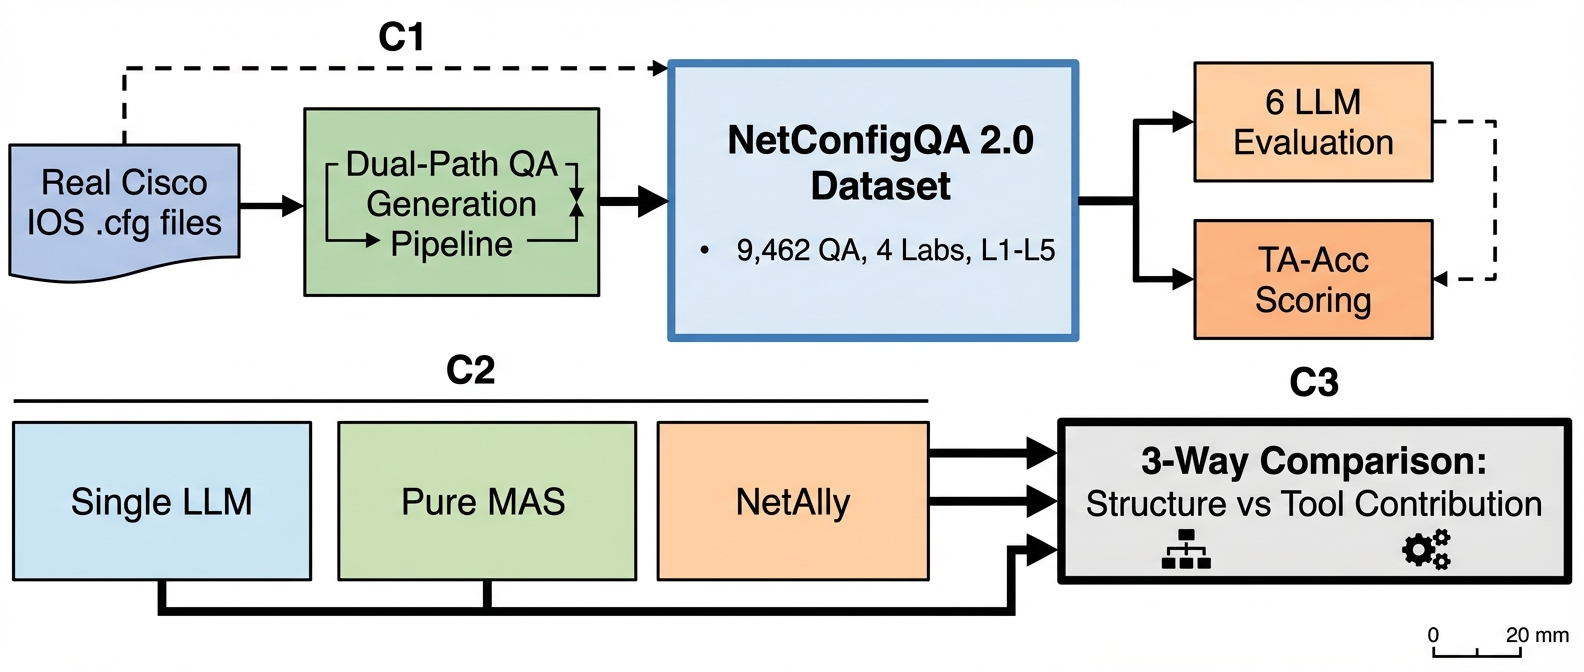
\includegraphics[width=0.7\textwidth]{figure/fig1_framework_overview_ai}
  \caption{연구 프레임워크 개요. 설정 파일로부터 QA를 자동 생성하는 벤치마크와 평가 지표로 LLM의 해석 능력을 평가하고(C1), 이 장벽을 우회하기 위한 도구 통합 시스템을 제시하며(C2), 3-way 비교를 통해 구조 효과와 도구 효과를 분리 분석한다(C3).}
  \label{fig:framework-overview}
\end{figure*}
\input{body/mas}

\section{Experiments}
\subsection{실험 설정}
평가 데이터셋은 NetConfigQA~2.0의 4개 Lab으로 구성되며, 전체 QA 수는 9,462개이다. 모델은 4개 벤더에서 6개 LLM을 선정하였다.

\begin{table*}[!t]
  \caption{평가 모델 구성}
  \label{tab:model-setup}
  \centering
  \small
  \begin{tabular}{|L{2.6cm}|L{2.0cm}|L{3.0cm}|L{1.8cm}|C{1.5cm}|}
    \hline
    \textbf{모델}   & \textbf{벤더} & \textbf{파라미터}       & \textbf{양자화} & \textbf{Context} \\
    \hline
    GPT-4o-mini   & OpenAI      & -- (API)            & --           & 128K             \\
    \hline
    GPT-OSS-20B   & OpenAI      & 20B                 & MXFP4        & 131K             \\
    \hline
    Qwen3-Coder   & Alibaba     & 30B MoE / 3B active & Q4\_K\_M     & 256K             \\
    \hline
    Gemma-3-27B   & Google      & 27B                 & Q4\_K\_M     & 128K             \\
    \hline
    GLM-4.7-Flash & Zhipu       & 30B MoE / 3B active & Q4\_K\_M     & 198K             \\
    \hline
    Qwen3.5-27B   & Alibaba     & 27B                 & Q4\_K\_M     & 262K             \\
    \hline
  \end{tabular}
\end{table*}

모든 평가는 zero-shot 조건에서 수행하며, temperature는 0으로 고정하고 `num\_ctx`는 49,152로 설정하였다. 로컬 모델 서빙은 RTX 3090 (24GB) 환경의 Ollama를 사용하였다. 평가 지표는 TA-Acc와 Format Stability(Parse Success Rate)이다. 모델 간 성능 차이의 유의성은 Bootstrap 95\% 신뢰구간(10,000회 리샘플링)으로 검정한다. Single LLM 평가가 완료되면 Overall TA-Acc가 가장 높은 오픈소스 모델을 Pure MAS와 NetAlly의 공통 backbone으로 사용한다([TODO]: 모델명).

\subsection{Single LLM 기준선과 확장성}
LLM의 설정 파일 해석 능력을 평가하기 위해 6개 모델을 4개 Lab에 각각 적용하여 총 $6\times4=24$회 평가하였다.

\begin{table*}[!t]
  \caption{Single LLM 기준선: Overall TA-Acc (6개 모델 $\times$ 4개 Lab). 각 셀은 Micro / Macro 순이다.}
  \label{tab:single-llm-baseline}
  \centering
  \small
  \begin{tabular}{|L{2.8cm}|C{1.9cm}|C{1.9cm}|C{1.9cm}|C{1.9cm}|}
    \hline
    \textbf{모델}   & \textbf{Lab-A (10)} & \textbf{Lab-B (20)} & \textbf{Lab-C (30)} & \textbf{Lab-D (40)} \\
    \hline
    GPT-4o-mini   & [TODO]              & [TODO]              & [TODO]              & [TODO]              \\
    \hline
    GPT-OSS-20B   & [TODO]              & [TODO]              & [TODO]              & [TODO]              \\
    \hline
    Qwen3-Coder   & [TODO]              & [TODO]              & [TODO]              & [TODO]              \\
    \hline
    Gemma-3-27B   & [TODO]              & [TODO]              & [TODO]              & [TODO]              \\
    \hline
    GLM-4.7-Flash & [TODO]              & [TODO]              & [TODO]              & [TODO]              \\
    \hline
    Qwen3.5-27B   & [TODO]              & [TODO]              & [TODO]              & [TODO]              \\
    \hline
  \end{tabular}
\end{table*}

파이프라인 확장성은 QA/노드 비율로 함께 보고한다. 본 데이터셋에서는 Lab-A 126, Lab-B 108, Lab-C 89, Lab-D 84로, 토폴로지 규모가 증가해도 QA 생성량이 동일한 수준에서 유지됨을 확인할 수 있다.

Table~\ref{tab:level-taacc}은 Lab-A에서의 레벨별 TA-Acc를 정리하기 위한 표이다. 이 표와 Fig.~\ref{fig:ta-acc-levels}는 모델이 어느 난이도 구간에서 성능 저하를 보이는지, 그리고 그 저하가 L3$\rightarrow$L4 구간에 집중되는지를 점검하는 데 사용한다. 본 연구는 설정 파일에 경로 계산에 필요한 정보가 존재함에도 그래프 기반 계산이 요구되는 시점에서 나타나는 성능 절벽을 \textbf{시뮬레이션 장벽(Simulation Barrier)}으로 지칭한다. 또한 결과 보고에서는 Micro와 Macro Average를 병행하여 레벨 불균형의 영향을 함께 제시한다. 예를 들어 Lab-A에서는 L4 비율이 11.6\%로 낮아 두 지표의 차이가 제한적일 수 있지만, L4 비율이 49\%인 Lab-D에서는 Micro Average가 L4에 더 크게 영향을 받을 수 있으므로 Macro Average를 함께 해석하는 것이 필요하다.

\begin{table*}[!t]
  \caption{Lab-A 레벨별 TA-Acc. Micro는 전체 QA 평균, Macro는 레벨별 평균의 산술 평균이다.}
  \label{tab:level-taacc}
  \centering
  \small
  \begin{tabular}{|L{2.4cm}|C{1.1cm}|C{1.1cm}|C{1.1cm}|C{1.1cm}|C{1.1cm}|C{1.3cm}|C{1.3cm}|}
    \hline
    \textbf{모델}   & \textbf{L1} & \textbf{L2} & \textbf{L3} & \textbf{L4} & \textbf{L5} & \textbf{Micro} & \textbf{Macro} \\
    \hline
    GPT-4o-mini   & --          & --          & --          & --          & --          & --             & --             \\
    \hline
    GPT-OSS-20B   & --          & --          & --          & --          & --          & --             & --             \\
    \hline
    Qwen3-Coder   & --          & --          & --          & --          & --          & --             & --             \\
    \hline
    Gemma-3-27B   & --          & --          & --          & --          & --          & --             & --             \\
    \hline
    GLM-4.7-Flash & --          & --          & --          & --          & --          & --             & --             \\
    \hline
    Qwen3.5-27B   & --          & --          & --          & --          & --          & --             & --             \\
    \hline
  \end{tabular}
\end{table*}

\begin{figure}[!t]
  \centering
  
\includegraphics[width=\columnwidth]{fig4_ta_acc_levels}
  \caption{Lab-A에서의 인지 난이도별 TA-Acc. 이 그림은 6개 모델의 레벨별 성능 분포를 비교하기 위한 것으로, 점선은 본 연구가 시뮬레이션 장벽으로 해석하는 L3$\rightarrow$L4 경계를 나타낸다.}
  \label{fig:ta-acc-levels}
\end{figure}

\begin{figure}[!b]
  \centering
  
\includegraphics[width=\columnwidth]{fig6_scalability}
  \caption{토폴로지 규모에 따른 레벨별 TA-Acc 변화. 이 그림은 노드 수 증가에 따라 각 레벨의 성능이 어떻게 달라지는지 비교하기 위한 것이다.}
  \label{fig:scalability}
\end{figure}

\subsection{구조 효과와 도구 효과: 3-Way 비교}
도구 통합을 통한 시뮬레이션 장벽의 우회 가능성을 확인하기 위해, Section~V-B에서 Overall TA-Acc가 가장 높은 오픈소스 모델을 선정하여 세 가지 설정을 비교한다.
\begin{itemize}
  \item \textbf{Single LLM:} 도구 없음, 설정 파일 전문을 프롬프트에 포함 (Section~V-B 결과 재사용)
  \item \textbf{Pure MAS:} Orchestrator + Executor 구조, 모든 도구 비활성화. L4/L5 질문에 대해 Executor는 도구 호출 없이 프롬프트에 포함된 설정 파일만으로 경로 추론을 시도한다.
  \item \textbf{NetAlly:} Orchestrator + Executor + Batfish/NSO/PNETLab 도구 활성화
\end{itemize}
세 설정의 공정한 비교를 위해 다음 변인을 통제한다: (1)~동일 LLM backbone (Section~V-B에서 선정된 모델), (2)~동일 시스템 프롬프트 기본 구조 (Pure MAS와 NetAlly는 스킬 가이드 주입 여부만 상이), (3)~동일 최대 토큰 예산 및 최대 추론 단계 (max\_steps = 10), (4)~동일 설정 파일 입력. Pure MAS와 Single LLM의 차이는 질문 분해(Orchestrator의 스킬 선택)와 다단계 추론(Executor의 ReAct 루프)에 한정되며, 두 설정 모두 외부 도구에 접근할 수 없다. Pure MAS와 NetAlly의 차이는 도구 바인딩의 활성화 여부만이다. 따라서 $\Delta$(구조) = Pure MAS $-$ Single은 에이전트 구조(질문 분해 + 다단계 추론)의 효과를, $\Delta$(도구) = NetAlly $-$ Pure MAS는 동일 구조에서 도구 통합의 효과를 각각 분리한다. 다만, $\Delta$(구조)에는 질문 분해와 컨텍스트 재구성이 혼재하므로 순수 ablation이 아닌 준실험(quasi-experiment) 설계임을 유의한다.

\begin{figure}[!t]
  \centering
  
\includegraphics[width=\columnwidth]{fig5_3way_comparison}
  \caption{Single LLM, Pure MAS, NetAlly의 3-way 비교. $\Delta$(구조)는 Single$\rightarrow$Pure MAS, $\Delta$(도구)는 Pure MAS$\rightarrow$NetAlly의 차이를 나타내며, 구조 효과와 도구 효과를 분리해 해석하기 위한 도식이다.}
  \label{fig:three-way}
\end{figure}

\begin{table*}[!t]
  \caption{3-way 비교 결과}
  \label{tab:three-way}
  \centering
  \small
  \begin{tabular}{|C{1.2cm}|C{2.0cm}|C{2.0cm}|C{2.0cm}|C{2.0cm}|C{2.0cm}|}
    \hline
    \textbf{레벨} & \textbf{Single} & \textbf{Pure MAS} & \textbf{NetAlly} & \textbf{$\Delta$(구조)} & \textbf{$\Delta$(도구)} \\
    \hline
    L1          & TBD             & TBD               & TBD              &                       &                       \\
    \hline
    L2          & TBD             & TBD               & TBD              &                       &                       \\
    \hline
    L3          & TBD             & TBD               & TBD              &                       &                       \\
    \hline
    L4          & TBD             & TBD               & TBD              &                       &                       \\
    \hline
    L5          & TBD             & TBD               & TBD              &                       &                       \\
    \hline
  \end{tabular}
\end{table*}

\begin{table*}[!t]
  \caption{도구 호출 분석}
  \label{tab:tool-call-analysis}
  \centering
  \small
  \begin{tabular}{|C{1.2cm}|L{4.0cm}|C{2.0cm}|C{2.0cm}|C{2.0cm}|}
    \hline
    \textbf{레벨} & \textbf{주요 도구}         & \textbf{호출 성공률} & \textbf{TA-Acc (성공)} & \textbf{TA-Acc (실패)} \\
    \hline
    L4          & Batfish traceroute     & TBD             & TBD                  & TBD                  \\
    \hline
    L5          & Batfish fork\_snapshot & TBD             & TBD                  & TBD                  \\
    \hline
  \end{tabular}
\end{table*}

\subsection{오류 분석}
L4/L5 오답은 무작위 표본을 추출하여 오류 유형별로 분류한다(Table~\ref{tab:error-analysis}). 분석의 목적은 단순 정확도 비교를 넘어, 모델이 어떤 지점에서 추론을 중단하거나 잘못된 경로를 구성하는지 정성적으로 파악하는 데 있다. 특히 빈 응답 또는 추론 회피, 추가 홉 오류, IP-노드 매핑 실패, 형식 오류, 컨텍스트 포화는 L4/L5 성능 저하를 해석하는 핵심 후보 유형으로 간주한다. 최종 원고에서는 각 유형의 비율과 대표 사례를 함께 제시할 예정이다.

\begin{table*}[!t]
  \caption{L4/L5 오류 유형 분류}
  \label{tab:error-analysis}
  \centering
  \small
  \begin{tabular}{|L{2.8cm}|C{2.0cm}|L{7.0cm}|}
    \hline
    \textbf{오류 유형} & \textbf{비율} & \textbf{근본 원인}                    \\
    \hline
    빈 응답 / 추론 회피   & TBD         & 경로 계산 자체를 시도하지 못하거나 ``확인 불가''로 회피 \\
    \hline
    추가 홉 오류        & TBD         & 3홉 이상에서 중간 노드 누락 또는 불필요한 노드 추가    \\
    \hline
    IP-노드 매핑 실패    & TBD         & 목적지 IP의 소속 장비를 파악하지 못해 경로 과연장     \\
    \hline
    형식 오류          & TBD         & path/set 포매팅 실패로 파싱 불가            \\
    \hline
    Context 포화     & TBD         & 대규모 config 입력 시 답변 퇴화             \\
    \hline
  \end{tabular}
\end{table*}
\section{Discussion}
\subsection{시뮬레이션 장벽의 원인}
Section~V-D의 오류 분석은 시뮬레이션 장벽이 정보의 부재가 아니라 \emph{계산의 불안정성}에서 비롯됨을 시사한다. 설정 파일에는 OSPF cost, BGP neighbor, 인터페이스 IP와 같이 경로 계산에 필요한 정보가 이미 포함되어 있다. 그러나 이러한 정보를 정답으로 변환하려면 다수 노드에 걸친 SPF 계산과 VRF별 포워딩 상태 구성이 필요하며, 이는 단순한 텍스트 회상과는 다른 계산적 추론을 요구한다. 토큰 예측 방식의 LLM은 이 과정에서 중간 단계 오류를 누적시키며, 그 결과는 주로 빈 응답과 추론 회피, 또는 중간 홉을 잘못 삽입하는 추가 홉 오류의 형태로 나타난다. 이러한 실패 패턴이 파라미터 규모와 아키텍처에 관계없이 반복된다는 점은, 본 연구가 관찰한 한계가 개별 모델의 성능 차이라기보다 토큰 예측 패러다임 자체의 구조적 제약에 가깝다는 해석을 뒷받침한다. Mondal et al.~\cite{ref30}이 GPT-4에서도 라우터 설정 합성에 검증기 피드백 루프가 필요하다고 보고한 결과는 이러한 관찰과 맥을 같이한다. 따라서 네트워크 운영 관점에서 L1\textasciitilde L3 수준의 사실 추출과 정적 확인에는 LLM을 직접 활용할 수 있지만, L4/L5 수준의 동작 추론에는 정형 분석 도구의 병행이 사실상 불가피하다.

\subsection{구조 효과와 도구 효과의 분리}
기존 연구~\cite{ref14, ref15}는 Multi-Agent 도입에 따른 성능 향상을 보고하지만, 그 향상의 원천이 에이전트 구조인지 연결된 도구인지까지는 분리해 설명하지 않는다. 이 구분은 시스템 설계 관점에서 중요하다. 만약 성능 향상의 핵심이 구조적 분업이 아니라 도구 접근성에 있다면, 복잡한 다중 에이전트 아키텍처를 구축하는 것보다 더 단순한 구조에 적절한 네트워크 분석 도구를 연결하는 편이 실용적으로 더 타당할 수 있기 때문이다.

본 연구의 3-way 비교는 바로 이 지점을 겨냥한다. $\Delta$(구조)는 도구 없이 에이전트 구조만 추가했을 때의 효과를, $\Delta$(도구)는 동일한 구조에 도구를 통합했을 때의 추가 효과를 나타낸다. L1\textasciitilde L3에서는 질문 분해와 답변 통합 과정이 일부 이점을 제공할 수 있으나, L4/L5에서는 하위 질문 자체가 traceroute나 what-if 분석과 같은 시뮬레이션 절차를 필요로 한다. 따라서 구조만으로는 한계를 넘기 어렵고, 실제 성능 개선은 도구 호출과 그 결과 해석이 결합될 때 비로소 나타난다. 이 구간에서 LLM의 역할은 직접적으로 경로를 계산하는 주체라기보다, 어떤 도구를 호출할지 선택하고 그 결과를 사용자 질의에 맞게 해석하는 조정자로 재정의된다.

\subsection{파이프라인의 범용성과 실용적 가치}
이중 경로 파이프라인은 특정 토폴로지에 종속되지 않도록 설계되었다. 4개 Lab에 동일한 생성 절차를 적용한 결과, 코드 수정 없이 메트릭 커버리지가 52\%(Lab-A)에서 97\%(Lab-D)까지 확장되었고, QA/노드 비율도 84\textasciitilde126 범위에서 비교적 안정적으로 유지되었다. 이는 파이프라인이 단일 예제에 맞춘 일회성 구성이라기보다, 토폴로지 규모와 프로토콜 구성이 바뀌더라도 유사한 방식으로 적용될 수 있음을 보여준다. 실무적으로는 운영 조직이 자사 설정 파일만 제공하더라도 LLM 기반 도구의 사전 성능 평가, 변경 이후의 회귀 테스트, 또는 특정 운영 태스크에 대한 위험 점검에 이 프레임워크를 활용할 수 있다.

\subsection{타당성 위협}
\textbf{벤더 종속성.} 실험은 Cisco IOS로 한정하였다. 이는 벤더 간 구문 차이와 운영 관례의 영향을 배제하여 비교 조건을 단순화하기 위한 선택이다. Batfish가 벤더 독립적 데이터 모델을 사용하므로 파이프라인과 난이도 체계 자체는 Juniper JUNOS나 Arista EOS로 확장 가능하지만, 본 논문의 결과는 우선 Cisco IOS 환경에서 해석하는 것이 적절하다.

\textbf{Ground Truth 독립성.} L4/L5의 Ground Truth와 NetAlly의 핵심 추론 도구가 모두 Batfish에 의존하므로, NetAlly의 L4/L5 정확도는 부분적으로 ``올바른 Batfish API를 적절한 파라미터로 호출했는가''를 반영한다. 본 연구는 이러한 순환성을 통제하기 위해 세 가지 조치를 취하였다. 첫째, PNETLab 실장비 CLI와의 교차 검증으로 Batfish 출력의 신뢰성을 확인하였다(Section~III-E, Method~3). 둘째, 순환성에서 자유로운 L1\textasciitilde L3에서도 유사한 성능 격차 패턴이 나타나는지 함께 확인하였다. 셋째, 도구 호출 성공/실패별 TA-Acc를 분리 보고하여(Table~\ref{tab:tool-call-analysis}) ``API 호출 성공''과 ``추론 품질''을 구분하고자 하였다. 다만 Batfish 외의 독립 오라클, 예를 들어 실장비 기반 대규모 자동 검증을 통한 완전한 순환 해소는 향후 과제로 남아 있다.

\textbf{토폴로지 규모.} 본 연구의 최대 규모는 40노드로, 대규모 엔터프라이즈나 통신사업자 환경 전체를 대표하기에는 제한적이다. 그럼에도 QA/노드 비율이 비교적 안정적으로 유지되었고 Config Generator가 임의 규모의 토폴로지를 지원한다는 점은, 본 접근이 더 큰 환경으로 확장될 가능성을 보여준다. 다만 그 확장이 실제로 어떤 비용과 성능 저하를 수반하는지는 후속 실험으로 확인할 필요가 있다.

\section{Conclusion}
본 논문에서는 ``LLM은 네트워크 설정 파일을 얼마나 정확하게 해석하고 분석할 수 있는가?''라는 질문에 답하기 위해 벤치마크 NetConfigQA~2.0, 평가 지표 TA-Acc, 도구 통합 Multi-Agent 시스템 NetAlly를 제안하였다. 이중 경로 파이프라인은 설정 파일만으로 QA를 자동 생성하였으며, 4개 토폴로지(10-40 노드, 9,473 QA)에 코드 수정 없이 적용되었고 3중 GT 검증에서 98-99.9\%의 일치율을 보였다. 6개 LLM을 평가한 결과, 사실 추출(L1-L3)에서는 모델 간 뚜렷한 성능 차이가 나타났으나 경로 추론과 장애 분석(L4-L5)에서는 모든 모델이 시뮬레이션 장벽에 직면하였다. 3-way 비교에서 MAS 구조만으로는 L4/L5가 개선되지 않았으나 네트워크 도구 통합 시 유의미한 변화가 관찰되어, 성능 향상의 주된 원천이 도구 통합에 있음을 확인하였다. TA-Acc는 BERTScore와 Exact Match가 구분하지 못하는 모델 간 차이를 식별하였다.

우리는 향후 연구로 L6 트러블슈팅 확장, 멀티 벤더(Juniper, Arista) 지원, 설정 생성 태스크 평가, 외부 벤치마크와의 교차 적용을 계획한다.




%  appendix 부분은 우선 주석 처리


% \appendices
% \section{Proof of the First Zonklar Equation}
% Appendix one text goes here.

% % you can choose not to have a title for an appendix
% % if you want by leaving the argument blank
% \section{}
% Appendix two text goes here.


% % use section* for acknowledgment
% \section*{Acknowledgment}


% The authors would like to thank...


% % Can use something like this to put references on a page
% % by themselves when using endfloat and the captionsoff option.
% \ifCLASSOPTIONcaptionsoff
%   \newpage
% \fi


% \begin{thebibliography}{1}

% \bibitem{IEEEhowto:kopka}
% H.~Kopka and P.~W. Daly, \emph{A Guide to \LaTeX}, 3rd~ed.\hskip 1em plus
%   0.5em minus 0.4em\relax Harlow, England: Addison-Wesley, 1999.

% \end{thebibliography}

% \begin{IEEEbiography}{Michael Shell}
% Biography text here.
% \end{IEEEbiography}

% % if you will not have a photo at all:
% \begin{IEEEbiographynophoto}{John Doe}
% Biography text here.
% \end{IEEEbiographynophoto}


% \begin{IEEEbiographynophoto}{Jane Doe}
% Biography text here.
% \end{IEEEbiographynophoto}

\bibliographystyle{IEEEtran}
\bibliography{reference}
\end{document}


